%!TEX root = ../tesi.tex

\chapter{Design Pattern}
\label{a:designpatterns}
Nel campo dell'Ingegneria del Software con Design Pattern si intende uno schema di progettazione del software utilizzato per risolvere un problema ricorrente.
Molti di questi schemi sono stai pensati per il paradigma di programmazione ad oggetti e descrivono, utilizzando ereditarietà e interfacce, le interazioni e relazioni tra oggetti e classi.

In questa appendice vengono esposte alcune note generali sui design pattern citati nel testo, sia che siano stati implementati direttamente o semplicemente coinvolti nello sviluppo del progetto di tesi perché sfruttati dalle parti interessate del framework.
Nella trattazione viene descritto l'obbiettivo di ogni schema, l'utilità, note implementative  e alcuni benefici della sua applicazione, vengono inoltre raggruppati per categoria così come vengono presentati in \cite{book:designpattern}.

\section{Pattern Creazionali}
I pattern creazionali sono usati per creare un'astrazione sul processo di instanziazione degli oggetti, in modo da rendere il sistema indipendente da come gli oggetti vengono effettivamente creati. Questo tipo di pattern diviene importante quando un sistema dipende principalmente da oggetti composti da aggregati di componenti più piccole, rispetto ad oggetti gerarchici organizzati in base all'ereditarietà.

\subsection{Abstract Factory}
\label{sub:abstractfactory}
L'obbiettivo di questo pattern è fornire un'interfaccia per la creazione di famiglie di oggetti imparentati o dipendenti tra loro, eliminado la necessità di specificare i nomi delle classi concrete all'interno del codice.

In questo modo un sistema può essere indipendente da come vengono creati gli oggetti concreti e può essere configurato per utilizzare diverse famiglie di oggetti a seconda delle necessità. Un caso esemplificativo è quello di un tool per l'implementazione di interfacce grafiche che supporta diversi look-and-feel. L'utilizzo di un diverso look-and-feel comporta la definizione di una nuova famiglia di componenti grafiche le cui caratteristiche base sono però fondamentalmente identiche: un pulsante può essere premuto e disegnato a schermo. L'applicazione dovrebbe essere appunto indipendente da come il pulsante viene istanziato, ma essere in grado di riconoscerlo per le sue funzionalità.

Per ottenere ciò è possibile definire una classe astratta o un'interfaccia differente per ogni componente generico desiderato.
Si definisce poi una classe Factory astratta la cui funzione sia quella di creare istanze delle componenti astratte generiche. Se per ogni famiglia che si desidera implementare si generano sottoclassi concrete per ogni componente astratta e si definisce una Factory in grado di istanziarle, l'applicazione potrà utilizzare la Factory concreta che preferisce in modo del tutto indipendente da quale famiglia essa gestisce.

Questo schema permette di cambiare le famiglie di componenti in modo semplice e consente di isolare le classi concrete, dato che le componenti vengono utilizzate attraverso la loro interfaccia.

\subsection{Singleton}
\label{sub:singleton}
Lo scopo di questo pattern è garantire che di una determinata classe possa essere creata una unica istanza, fornendone un singolo punto di accesso globale.

L'utilità di questo pattern è dovuta al fatto che spesso, all'interno di un'applicazione, ci sono servizi e funzionalità condivise a cui deve essere associata una istanza univoca. Esempi classici in proposito sono il gestore del File System o il gestore dei servizi di stampa.

Per ottenere questa proprietà spesso si delega alla classe stessa la responsabilità di controllare la creazione delle propria istanza rendendo privato il suo costruttore, impedendo di fatto l'istanziazione dall'esterno.

Utilizzare questo schema consente di avere un più stretto controllo degli accessi alla risorsa, inoltre estendendo la classe è possibile raffinare le funzionalità della risorsa e configurare l'applicazione a runtime per utilizzare l'istanza che serve per un caso specifico.

\section{Pattern Strutturali}
Questo tipo di pattern si occupano di come classi e oggetti vengono composte e interagiscono nella formazione di strutture più complesse. 
Un obbiettivo di questi pattern è permettere la composizione di oggetti complessi che uniscano le funzionalità di moduli più piccoli rendendo quest'ultimi il più possibile riutilizzabili.

\subsection{Bridge}
\label{sub:bridge}
Questo pattern ha l'intento di disaccoppiare un'astrazione dalla sua implementazione in modo che entrambe possano evolversi in maniera indipendente.

Ciò è particolarmente utile quando si desidera evitare un legame permanente tra astrazione e implementazione, e si vuole permettere di scegliere o cambiare quest'ultima durante l'esecuzione. É utile inoltre quando sia astrazione che implementazione hanno la necessità di essere estendibili attraverso sottoclassi. 

Un utile esempio per illustrare questo pattern è prendere in esame un ipotetico toolkit per interfacce grafiche, per renderlo il più possibile portabile su piattaforme diverse esso deve utilizzare un'astrazione che descriva le finestre in modo più generico possibile. Se per ottenere queste proprietà usassimo semplicemente una classe astratta \texttt{Window} da cui, usando l'ereditarietà, costruire sottoclassi specifiche per ogni sistema da supportare, otterremmo due svantaggi:
\begin{enumerate}
	\item Nell'evenienza di voler estendere la classe \texttt{Window} per coprire l'astrazione di altri tipi di finestra grafica esistente, per poter supportare tutte le piattaforme per cui esisteva una implementazione di \texttt{Window} dovremmo creare una sottoclasse specifica per ognuna di esse.
	\item Il codice del client diventa dipendente dalla piattaforma. Quando vi è la necessità di creare una finestra, deve essere istanziata una classe concreta specifica e questo lega fortemente l'astrazione con l'implementazione utilizzata rendendo più complesso portare il codice del client su altre piattaforme.
\end{enumerate}
Per eludere questi problemi il pattern Bridge separa la gerarchia delle classi che appartengono all'astrazione da quella delle classi di implementazione. In cima alle due gerarchie vi sono le classi \texttt{Window} e \texttt{WindowImplementation}, che compongono il Bridge vero e proprio. La prima rappresenta l'astrazione della finestra che verrà utilizzata dal client, la seconda è invece l'interfaccia che un'implementazione concreta deve utilizzare per essere utilizzata dall'astrazione.
Come si può vedere nella figura \ref{f:bridgepattern}, la classe \texttt{Window} rimappa i propri metodi su quelli dell'interfaccia \texttt{WindowImplementation}, o con una combinazione di essi. Questi vengono chiamati su di una implementazione concreta di \texttt{WindowImplementation} di cui \texttt{Window} possiede un riferimento \texttt{imp}.

\begin{figure}
\begin{center}
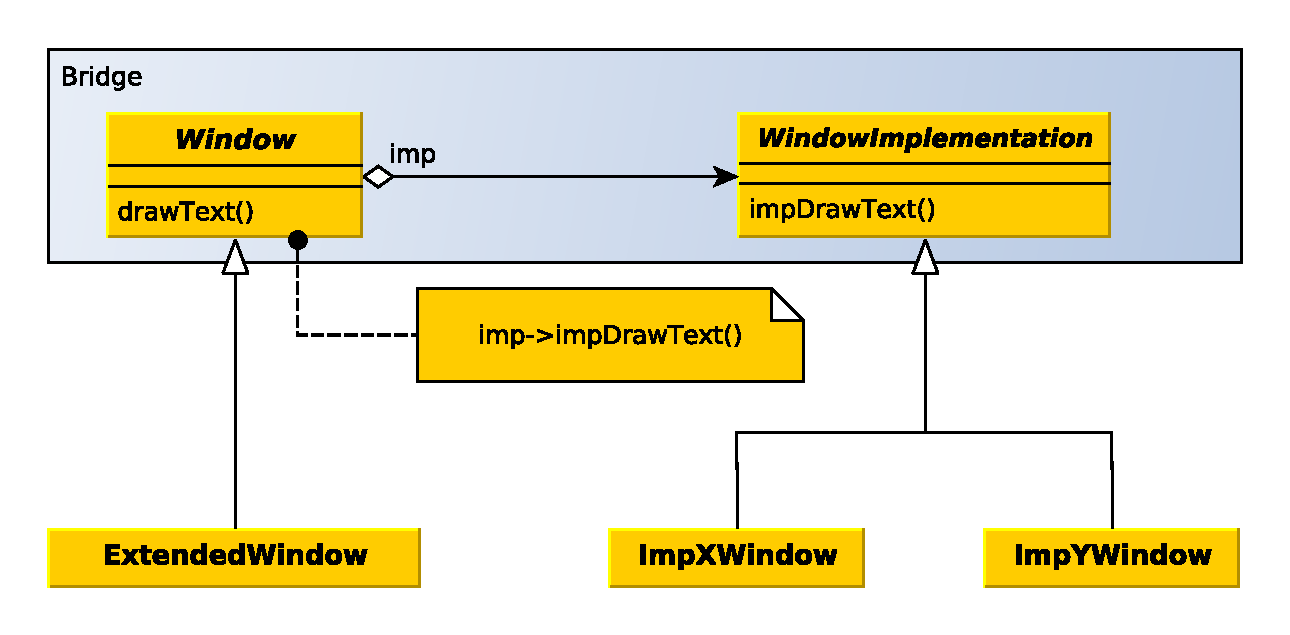
\includegraphics[width=12cm]{Immagini/BridgePattern}
\caption{Esempio di schema gerarchico dovuto all'applicazione del pattern Bridge.\label{f:bridgepattern}} 
\end{center} 
\end{figure}

L'utilizzo di questo schema permette di nascondere i dettagli implementativi ai client e di non avere effetti diretti su di esse quando l'implementazione cambia così che il codice dei client non non ha un'effettiva necessità di essere ricompilato. 

\subsection{Composite}
\label{sub:composite}
Lo scopo di questo pattern è consentire una gestione uniforme tra oggetti semplici ed oggetti compositi. Questo si traduce in una organizzazione degli oggetti in una struttura ad albero in cui ogni nodo è un oggetto aggregato e ogni foglia è un oggetto semplice.

Spesso si desidera poter trattare oggetti composti nello stesso modo in cui gestiamo le sue componenti ignorando come siano effettivamente implementate le loro funzionalità, un esempio significativo sono le interfacce grafiche in cui è comodo poter gestire gruppi di componenti, come pulsanti o etichette, in modo unitario come se si trattasse di una componente singola.

Una metodologia per ottenere questo tipo di interazione è l'utilizzo di una classe astratta che rappresenti sia gli oggetti semplici, o primitive, sia gli oggetti composti, o contenitori.

L'utilizzo di questo pattern consente di rendere meno complessi i moduli che utilizzano le strutture composite, che non hanno bisogno di sapere se stiano trattando una foglia o un nodo dell'albero. Consente inoltre di aggiungere in modo semplice nuovi componenti senza laboriosi interventi sul codice pre-esistente.
% TODO: valutare una citazione sul principio OpenClose SOLID